\input{"../../../preamble"}

\begin{document}

\title{CSC263-Notes-01-14-2015}

\input{"../csc263-header"}
\rhead{January 14, 2015}

\section*{Lecture 04}

\subsection*{Approaches to building a heap}

\begin{enumerate}[label={(\Alph*)}]
	\item sort the array using some other sorting algoritm - $O(n\log n)$
	\item start with empty heap, for each of the $n$ items, insert into a heap - $O(n\log n)$
	\item Heapify/Build Heap - Put the items randomly in the array and then ``correct''. Once the items are in an array (in any order) we can consider them a heap that has the corsdrect shape and then we have to fix the order - $O(n)$
\end{enumerate}

\subsection*{\texttt{heapify(A,i)}}

\noindent Given array $A$ representing a complete binary tree and element $x$ at position $i$ of $A (x=A[i])$ and assuming that the subtrees rooted at the children of $x$ are valid heaps, bubble-down $x$ such that the subtree rooted at $x$ is a valid heap.

\subsection*{\texttt{build-heap(A)}}

\begin{enumerate}[label={(\arabic*)}]
	\item put elements into array $A$ in any order
	\item call \texttt{build-heap(A)}
\end{enumerate}

\begin{lstlisting}[language=Python,mathescape]
build-heap(A):
	heapsize $\leftarrow$ size(A)
	for i in $\floor{\textrm{heapsize}/2} \ldots 1$:
		heapify(A,i)
\end{lstlisting}

\noindent Because each item in the second half of the array is already a heap (it's a leaf), the preconditions for \texttt{heapify} are always met before each call. Trace \texttt{build-heap} on input $A = [1,5,7,6,2,9,4,8]$: \\

\begin{tabular}{c @{ $\rightarrow$ } c @{ $\rightarrow$ }}

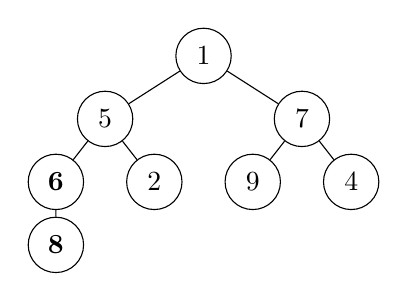
\begin{tikzpicture}[every node/.style={circle,draw,minimum size=2em,inner sep=1},
	baseline={(current bounding box.center)},
	level/.style={level distance=8mm,sibling distance=25mm/#1}]
\node {1}
child {node {5}
	child {node {\textbf{6}}
		child {node {\textbf{8}}}
		}
	child {node {2}}
	}
child {node {7}
	child {node {9}}
	child {node {4}}
	};
\end{tikzpicture} &

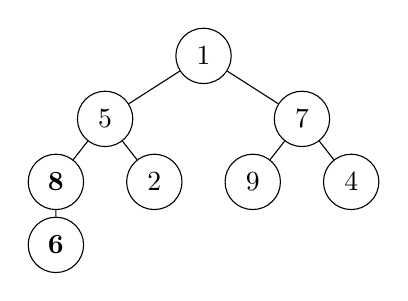
\begin{tikzpicture}[every node/.style={circle,draw,minimum size=2em,inner sep=1},
	baseline={(current bounding box.center)},
	level/.style={level distance=8mm,sibling distance=25mm/#1}]
\node {1}
child {node {5}
	child {node {\textbf{8}}
		child {node {\textbf{6}}}
		}
	child {node {2}}
	}
child {node {7}
	child {node {9}}
	child {node {4}}
	};
\end{tikzpicture} \\

\texttt{heapify([1,5,7,\textbf{6},2,9,4,\textbf{8}], 4)} & \texttt{[1,5,7,\textbf{8},2,9,4,\textbf{6}]} \\

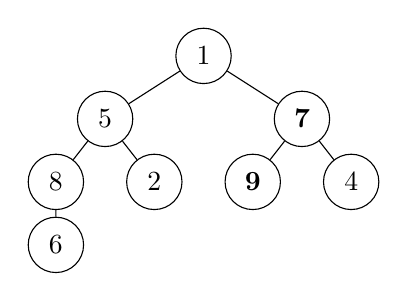
\begin{tikzpicture}[every node/.style={circle,draw,minimum size=2em,inner sep=1},
	baseline={(current bounding box.center)},
	level/.style={level distance=8mm,sibling distance=25mm/#1}]
\node {1}
child {node {5}
	child {node {8}
		child {node {6}}
		}
	child {node {2}}
	}
child {node {\textbf{7}}
	child {node {\textbf{9}}}
	child {node {4}}
	};
\end{tikzpicture} &

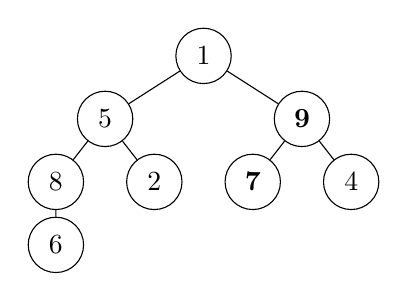
\begin{tikzpicture}[every node/.style={circle,draw,minimum size=2em,inner sep=1},
	baseline={(current bounding box.center)},
	level/.style={level distance=8mm,sibling distance=25mm/#1}]
\node {1}
child {node {5}
	child {node {8}
		child {node {6}}
		}
	child {node {2}}
	}
child {node {\textbf{9}}
	child {node {\textbf{7}}}
	child {node {4}}};
\end{tikzpicture} \\

\texttt{heapify([1,5,\textbf{7},8,2,\textbf{9},4,6], 3)} & \texttt{[1,5,\textbf{9},8,2,\textbf{7},4,6]} \\

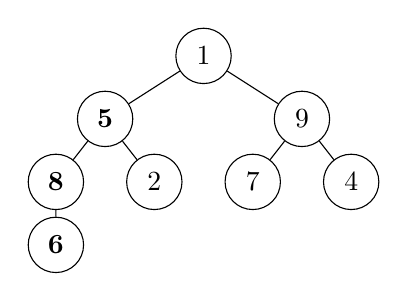
\begin{tikzpicture}[every node/.style={circle,draw,minimum size=2em,inner sep=1},
	baseline={(current bounding box.center)},
	level/.style={level distance=8mm,sibling distance=25mm/#1}]
\node {1}
child {node {\textbf{5}}
	child {node {\textbf{8}}
		child {node {\textbf{6}}}
		}
	child {node {2}}
	}
child {node {9}
	child {node {7}}
	child {node {4}}};
\end{tikzpicture} &

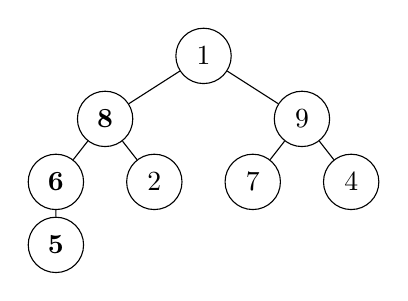
\begin{tikzpicture}[every node/.style={circle,draw,minimum size=2em,inner sep=1},
	baseline={(current bounding box.center)},
	level/.style={level distance=8mm,sibling distance=25mm/#1}]
\node {1}
child {node {\textbf{8}}
	child {node {\textbf{6}}
		child {node {\textbf{5}}}
		}
	child {node {2}}
	}
child {node {9}
	child {node {7}}
	child {node {4}}};
\end{tikzpicture} \\

\texttt{heapify([1,\textbf{5},9,\textbf{8},2,7,4,\textbf{6}], 2)} & \texttt{[1,\textbf{8},9,\textbf{6},2,7,4,\textbf{5}]} \\

\end{tabular}

\begin{tabular}{c @{ $\rightarrow$ } c}

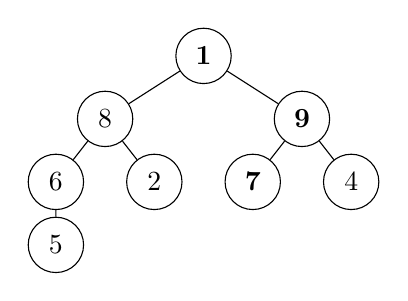
\begin{tikzpicture}[every node/.style={circle,draw,minimum size=2em,inner sep=1},
	baseline={(current bounding box.center)},
	level/.style={level distance=8mm,sibling distance=25mm/#1}]
\node {\textbf{1}}
child {node {8}
	child {node {6}
		child {node {5}}
		}
	child {node {2}}
	}
child {node {\textbf{9}}
	child {node {\textbf{7}}}
	child {node {4}}};
\end{tikzpicture} &

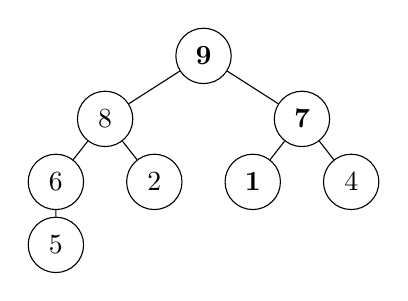
\begin{tikzpicture}[every node/.style={circle,draw,minimum size=2em,inner sep=1},
	baseline={(current bounding box.center)},
	level/.style={level distance=8mm,sibling distance=25mm/#1}]
\node {\textbf{9}}
child {node {8}
	child {node {6}
		child {node {5}}
		}
	child {node {2}}
	}
child {node {\textbf{7}}
	child {node {\textbf{1}}}
	child {node {4}}};
\end{tikzpicture} \\

\texttt{heapify([\textbf{1},8,\textbf{9},6,2,\textbf{7},4,5], 1)} & \texttt{[\textbf{9},8,\textbf{7},6,2,\textbf{1},4,5]} \\

\end{tabular}

\subsection*{Complexity of Build Heap}

\noindent We make $O(n)$ calls to \texttt{heapify} and each takes $O(\log n)$ time, so we immidiately get a bound of 
	$O(n \log n)$. But we can do better by analyzing more carefully. The running time of each call to \texttt{heapify}
	is proportional to the height of the tree on which it is called. So we get that the total time taken is 
$$O \left (\sum_{h=1}^{\log n} h \cdot a \right ) \textrm{ where } a= \textrm{ \# of subtrees of height }h$$

\noindent How many subtrees of each height? \\

\begin{tabular}{l}
	1 node at height $\log (n)$ \\
	2 nodes at height $\log (n) -1$ \\
	$\vdots$ \\
	$n/8$ nodes at height 2 (requiring at most 2 swaps)\\
	$n/4$ nodes at height 1 (requiring at most 1 swap)\\
	$n/2$ nodes at height 0 (require 0 swaps) \\
\end{tabular} \\

\noindent A complete tree with $n$ nodes contains at most
$\left \lceil \frac{n}{2^{h+1}} \right \rceil$
subtrees of height $n$.\\

\noindent Since a complete tree with $n$ nodes contains at most $\left \lceil \frac{n}{2^{h+1}} \right \rceil$ nodes of height $h$, we get that the running time of \texttt{build-heap} is

\mymarginpar{\textit{Note:}$$\sum_{k=0}^\infty \frac{k}{2^k} = 2$$}

$$O \left (\sum_{h=1}^{\log n} h \left \lceil \frac{n}{2^{h+1}} \right \rceil \right ) \leq 
O \left (\frac{n}{2} \sum_{h=1}^{\infty} \frac{h}{2^h} \right )=
O(n)$$

\noindent The 2 in the denominator comes from the previous $h+1$ that was simplified to $h$ but this doesn't matter in light of asymptotic analysis.

\subsection*{\texttt{heap-sort}}

\noindent Starting from an array $A$ in some arbitrary order, we must start by building a heap from $A$, using the process just described. Then, set heapsize == size of $A$ and repeatedly:
\begin{itemize}
	\item swap the root and the element at position heapsize (which means that the element that ends up at position heapsize is in the correct sorted position)
	\item decrement heapsize (since the last element is not part of the heap anymore)
	\item \texttt{heapify} starting at the root
\end{itemize} 
This last repeated step should look familiar. It is simply calling \texttt{extractMax} repeatedly from the heap until it is empty.\\

\noindent The complexity of \texttt{heap-sort}
$$\Theta(n \log n)$$
since we \texttt{extractMax} $n$ times and each call is $O(\log n)$.
\end{document}